\chapter{Elettrocardiografia e basi elettrofisiologiche}

\section{Anatomia ed elettrofisiologia del Cuore}
Il cuore è un organo muscolare cavo situato nel mediastino, leggermente spostato a sinistra. Ha il compito di distribuire il sangue (ossigenato e non) in tutto il nostro corpo.

Il cuore è diviso in quattro camere principali: atrio destro e sinistro, ventricolo destro e sinistro; gli atri sono posti nella parte superiore e hanno il compito di raccogliere il sangue e pomparlo dentro i ventricoli, questi ultimi sono le cavità più grandi e hanno il compito di pompare il sangue ognuno nelle proprie circolazioni: circolazione polmonare per il ventricolo destro e circolazione sistemica per il ventricolo sinistro.

\begin{center}
\begin{tabular}{>{\bfseries}l l l}
\toprule
Camera & Funzione & Vasi associati \\
\midrule
Atrio destro   & Raccoglie il sangue venoso sistemico  & Vene cave superiore e inferiore \\
Ventricolo destro & Pompa il sangue verso i polmoni    & Arteria polmonare \\
Atrio sinistro & Raccoglie il sangue ossigenato        & Vene polmonari \\
Ventricolo sinistro & Pompa il sangue verso il corpo   & Aorta \\
\bottomrule
\end{tabular}
\end{center}  
\begin{figure}[h!]
    \centering
    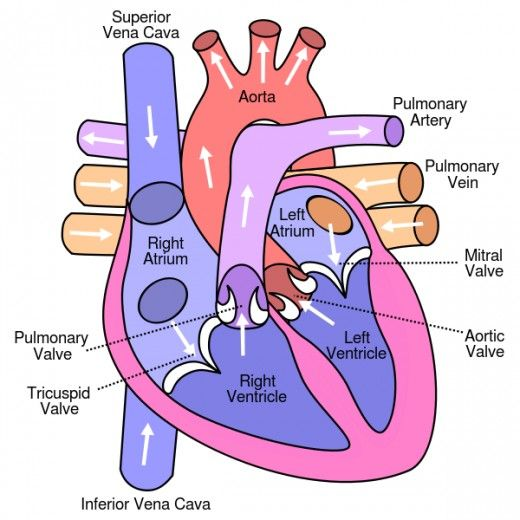
\includegraphics[width=0.6\linewidth]{images/heart.jpg}
    \caption{Foto del cuore con vene e arterie principali, presenti anche le valvole atrioventricolari e semilunari}
    \label{fig:placeholder}
\end{figure}
In ogni punto di comunicazione all'interno del cuore sono presenti delle valvole; esse garantiscono il flusso unidirezionale del sangue impedendone il reflusso. Le valvole si distinguono in due gruppi funzionali:

\begin{itemize}
  \item \textbf{Valvole atrioventricolari: (VA)} ancorate ai muscoli papillari del ventricolo tramite le \textit{corde tendinee}, che impediscono il prolasso dei lembi durante la sistole ventricolare; sono presenti due valvole di questo tipo: la \textit{valvola tricuspide}, posta tra atrio e ventricolo destro, è composta da tre lembi, e la \textit{valvola mitrale} (o bicuspide), posta tra tra atrio e ventricolo sinistro e composta da due lembi. 
  \item \textbf{Valvole semilunari:} prive di corde tendinee, si aprono e chiudono passivamente in risposta al gradiente di pressione. Abbiamo la \textit{valvola semilunare polmonare}, posta tra ventricolo destro e arteria polmonare, e la \textit{valvola semilunare aortica}, posta tra ventricolo sinistro e aorta.
\end{itemize}

\subsection{La parete cardiaca}

La parete del cuore è costituita da tre strati concentrici:
\begin{itemize}
  \item \textbf{Endocardio}: lo strato più interno, formato da tessuto endoteliale; riveste le cavità cardiache e le valvole.
  \item \textbf{Miocardio}: lo strato intermedio e più spesso, composto da cellule muscolari striate di tipo cardiaco (\textit{cardiomiociti}); è responsabile della forza contrattile del cuore. Lo spessore varia a seconda della camera: è massimo nel ventricolo sinistro, che deve vincere la resistenza della circolazione sistemica.
  \item \textbf{Epicardio}: lo strato più esterno, costituito da mesotelio e tessuto connettivo; corrisponde al \textit{foglietto viscerale} del pericardio sieroso.
\end{itemize}

Il cuore è poi avvolto esternamente dal \textbf{pericardio}, una sacca a doppia parete composta da:

\begin{itemize}
  \item \textbf{Pericardio fibroso}: lo strato esterno, robusto e inestensibile, che ancora il cuore al mediastino e lo protegge da sovradistensioni.
  \item \textbf{Pericardio sieroso}: suddiviso a sua volta in:\textit{Foglietto parietale} che riveste internamente il pericardio fibroso e il \textit{Foglietto viscerale} (o epicardio) che aderisce direttamente alla parete cardiaca.
\end{itemize}

Tra i due foglietti del pericardio sieroso è presente la \textbf{cavità pericardica}, che contiene una piccola quantità di liquido sieroso ($\sim$20--50 mL) con funzione lubrificante, riducendo l'attrito durante i movimenti del cuore.

\subsection{Contrazione e composizione cellulare}
Il cuore è composto principalmente da \textbf{cardiomiociti}, cellule 
muscolari striate specializzate che si contraggono involontariamente 
per pompare il sangue. Queste cellule sono connesse tramite i 
\textbf{dischi intercalari}, strutture che contengono desmosomi, 
utilizzati per l'ancoraggio meccanico, e \textbf{giunzioni gap}, canali che 
permettono il passaggio diretto di ioni tra cellule adiacenti, 
garantendo una propagazione rapida dell'impulso elettrico.
\begin{figure}[h!]
    \centering
    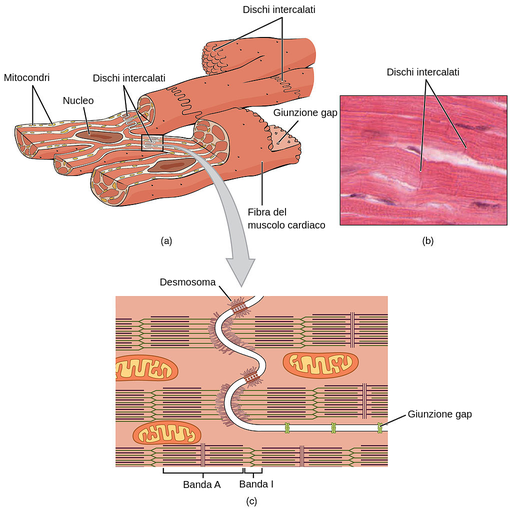
\includegraphics[width=0.33\linewidth]{images/cardiomicito.png}
    \caption{cardiomicito}
    \label{fig:cardiomicito}
\end{figure}

L'impulso viene generato dalle \textbf{cellule nodali}, in gergo \textit{pacemaker}, che a differenza dei cardiomiociti non si contraggono, ma sono specializzate nella generazione del segnale elettrico. Queste cellule sono raggruppate nell'atrio destro in prossimità della vena cava superiore, nel \textbf{nodo senoatriale (SA)}, e hanno la capacità di depolarizzarsi spontaneamente e ritmicamente, dando origine a ogni battito cardiaco. L'impulso generato viene poi irradiato in tutto il cuore tramite un sistema di conduzione composto da fibre di conduzione.
\begin{figure}[h!]
    \centering
    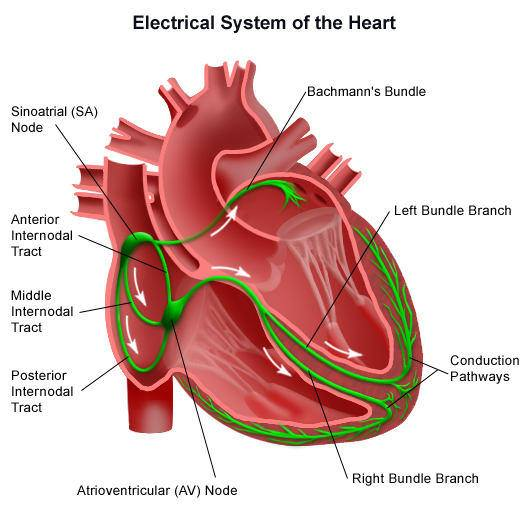
\includegraphics[width=0.3\linewidth]{images/sistema-elettrico-del-cuore.jpg}
    \caption{sistema di conduzione del cuore}
    \label{fig:sist-cond-cuore}
\end{figure}

\subsection{Il Ciclo Cardiaco}

Il ciclo cardiaco rappresenta la sequenza di eventi meccanici ed elettrici che si ripete ad ogni battito. A riposo, per un adulto medio, la frequenza cardiaca è di circa \textbf{60--80 battiti/min}, per cui ogni ciclo dura circa \textbf{800\,ms}. Ogni ciclo cardiaco è formato da due azioni principali: sistole (contrazione) e diastole (rilassamento).

\subsubsection{Prima fase}
La prima fase del ciclo cardiaco è per convenzione la \textbf{sistole atriale}, che spinge il sangue dagli atri nei ventricoli. Questa fase ha una durata di circa 100 ms, alla fine della quale, inizia la \textbf{diastole atriale} che durerà fino all'inizio del prossimo ciclo cardiaco.

\subsubsection{Seconda fase}
La seconda fase è invece la \textbf{sistole ventricolare}, questa ha una durata di circa 270 ms e suddivide ulteriormente in due sotto-fasi: 
\begin{itemize}
    \item \textbf{fase isovolumetrica}: dove la pressione spinge le valvole AV a chiudersi, ma non ne crea abbastanza per aprire le valvole semilunari.
    \item \textbf{fase propulsiva}: la pressione aumenta e supera quella delle arterie, le valvole semilunari si aprono e il sangue viene espulso.
\end{itemize}

\subsubsection{Terza fase}
Qui avviene l'ultima fase del ciclo cardiaco, la \textbf{diastole ventricolare}; anch'essa divisa in due sotto-fasi:
\begin{itemize}
    \item \textbf{fase precoce}: la pressione ventricolare inizia a calare, parte del sangue refluisce verso le valvole semilunari, chiudendole. Il sangue inizia a fluire negli atri rilasciati.
    \item \textbf{fase tardiva}: la diminuzione della pressione nei ventricoli apre le valvole AV, permettendo un riempimento passivo dei ventricoli.
\end{itemize}

\subsection{Elettrofisiologia}
Lo standard per l'elettrocardiogramma (ECG) è a dodici derivazioni, esse sono generate da 10 elettrodi posizionati sulla cute in specifici punti; prima di parlare di ECG, andiamo a vedere che cosa misuriamo effettivamenti tramite gli elettrodi.

\subsubsection{Potenziale di membrana}

I cardiomiociti, come tutte le cellule muscolari, mantengono a riposo un \textbf{potenziale di membrana negativo}, pari a circa \textbf{-90\,mV}; ed è proprio grazie a questo squilibrio elettrico che la cellula è in grado di contrarsi. Il potenziale negativo a riposo rappresenta infatti uno \textit{stato di carica}, come un condensatore pronto a scaricarsi: quando arriva il segnale elettrico appropriato, la cellula può depolarizzarsi rapidamente e innescare la contrazione muscolare.

\begin{figure}[h!]
    \centering
    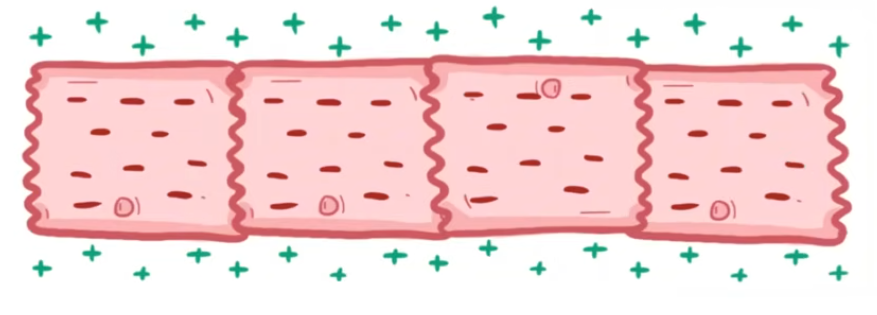
\includegraphics[width=0.4\linewidth]{images/potenziale-riposo-cardiomicito.png}
    \caption{Potenziale a riposo di un cardiomiocito}
    \label{fig:placeholder}
\end{figure}

Questo potenziale negativo viene mantenuto dalla naturale distribuzione asimmetrica degli ioni tra l'interno e l'esterno della cellula: gli ioni $K^+$ sono presenti in alta concentrazione \textit{all'interno}, mentre gli ioni $Na^+$ si trovano in alta concentrazione \textit{all'esterno}. Questa asimmetria, tuttavia, tende naturalmente a degradarsi. 

Gli ioni $K^+$, seguendo il loro gradiente di concentrazione, fuoriescono dalla cellula attraverso un canale passivo chiamato \textbf{Kir} (canale a rettificazione interna). Poiché ogni ione $K^+$ che esce porta con sé una carica positiva, l'interno della cellula diventa progressivamente più negativo contribuendo al potenziale di riposo, ma impoverendo la cellula di $K^+$.Per contrastare questa perdita e mantenere stabile la distribuzione ionica, entra in gioco la \textbf{pompa Na/K-ATPasi}. Si tratta di una pompa \textit{attiva}, che consuma energia sotto forma di ATP, che lavora \textit{contro gradiente} trasportando simultaneamente:

\begin{itemize}
    \item \textbf{3 ioni $Na^+$} verso l'esterno,
    \item \textbf{2 ioni $K^+$} verso l'interno.
\end{itemize}

In questo modo, la pompa ripristina continuamente le concentrazioni ioniche, mantenendo l'interno ricco di $K^+$ e l'esterno ricco di $Na^+$ e con esse, il potenziale di membrana negativo che rende possibile la contrazione.

\subsubsection{Fasi della contrazione}
Quando arriva lo stimolo generato dalle cellule nodali, il cardiomiocita attraversa un ciclo elettrico suddiviso in cinque fasi (da 0 a 4).

\begin{description}
    \item[Fase 0 -- Depolarizzazione rapida] 
    Lo stimolo provoca l'apertura dei canali voltaggio-dipendenti del $Na^+$, una grande quantità di ioni $Na^+$ entra all'interno della cellula, portando cariche positive all'interno. Il potenziale di membrana passa rapidamente da $-90$ mV a circa $+30$ mV. Questo processo, in cui la cellula perde la sua polarità negativa interna, prende il nome di \textbf{depolarizzazione}.

    \item[Fase 1 -- Ripolarizzazione iniziale]
    I canali del $Na^+$ si inattivano e gli ioni $K^+$ iniziano a muoversi verso gradiente tramite i canali passivi \textbf{Kir}, la fuoriuscita provoca una breve e parziale ripolarizzazione della membrana.

    \item[Fase 2 -- Plateau]
    Si apre una corrente di ioni $Ca^{2+}$ attraverso i canali di tipo L, la cui carica positiva in entrata \textbf{bilancia} la fuoriuscita di $K^+$, mantenendo il potenziale di membrana su un valore pressoché stabile per circa 200 ms. Questa fase è fondamentale perché l'ingresso di $Ca^{2+}$ permetta la contrazione del cardiomiocita.

    \item[Fase 3 -- Ripolarizzazione rapida]
    I canali del $Ca^{2+}$ si chiudono mentre i canali del $K^+$ rimangono 
    aperti: la fuoriuscita massiva di $K^+$ riporta il potenziale di 
    membrana rapidamente verso i valori di riposo.

    \item[Fase 4 -- Riposo]
    Il potenziale di membrana si stabilizza a $-90$ mV. La pompa $Na$/$K$ ripristina attivamente le concentrazioni ioniche originali, facendo uscire i $Na^+$ e reintroducendo $K^+$. Il processo opposto alla depolarizzazione, ovvero il ripristino della polarità negativa interna, prende il nome di \textbf{ripolarizzazione}.

\end{description}

\begin{figure}[h!]
    \centering
    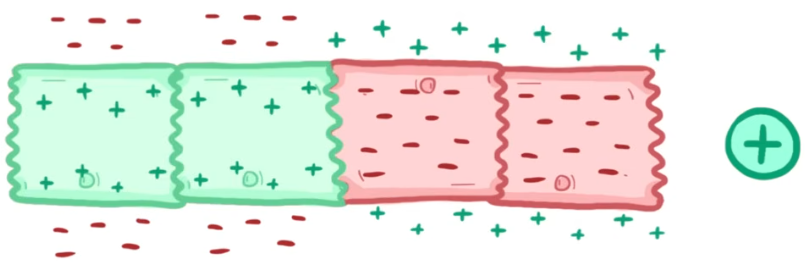
\includegraphics[width=0.4\linewidth]{images/onda-depolarizzazione.png}
    \caption{Onda di depolarizzazione, verso destra}
    \label{fig:placeholder}
\end{figure}

La cosa fondamentale è che la propagazione dello stimolo non avviene istantaneamente su tutte le cellule, ma si propaga nel tempo tramite le \textit{giunzioni gap}. Questa zona di confine tra la parte depolarizzata e quella ancora a riposo viene chiamata \textbf{fronte di depolarizzazione}. In corrispondenza di tale fronte si crea un \textbf{dipolo}, ed è proprio questo a generare il campo elettrico che poi si espanderà fino alla superficie del nostro corpo. Il verso del dipolo segue il verso di propagazione del fronte.

\section{ECG a 12 derivazioni}

Gli elettrodi sono dei trasduttori e hanno il compito di misurare le differenze di potenziale sulla superficie corporea, generate dalle correnti ioniche che scorrono all'interno del sistema di conduzione del cuore. 

Un elettrodo misura solamente i campi elettrici generati dall'onda di depolarizzazione, che sono diretti verso di esso, ad esempio, se rispetto all'elettrodo, il cardiomiocito è angolato di 45°, dovremmo dividere il vettore del campo in 2 parti e prendere quella nella direzione dell'elettrodo. Questo è il motivo per il quale abbiamo bisogno di relativamente tanti elettrodi in posti diversi per analizzare in modo adeguato il funzionamento del cuore.

\subsection{Posizionamento degli elettrodi}
\label{pos_elettrodi}
Come spiegato precedentemente, gli elettrodi fisici che devono essere posizionati sul corpo sono dieci: \textbf{6 precordiali}, posizionati nello spazio intercostale sul piano trasversale (foto di destra), più precisamente abbiamo: \textit{V1} sul quarto spazio intercostale linea parasternale destra, \textit{V2} quarto spazio intercostale linea parasternale sinistra, \textit{V3} a metà strada tra \textit{V2} e \textit{V4}, \textit{V4} quinto spazio intercostale linea emiclaveare sinistra, \textit{V5} quinto spazio intercostale linea ascellare anteriore sinistra e \textit{V6} quinto spazio intercostale linea ascellare media sinistra, e \textbf{4 periferici}, i 2 superiori sono solitamente posizionati nella spalla o nel polso mentre i 2 inferiori nella caviglia o nella gamba (foto di sinistra). 

Nel grafo dell'ECG abbiamo dodici derivazioni, di cui nove unipolari e tre bipolari:
\begin{figure}[h!]
    \centering
    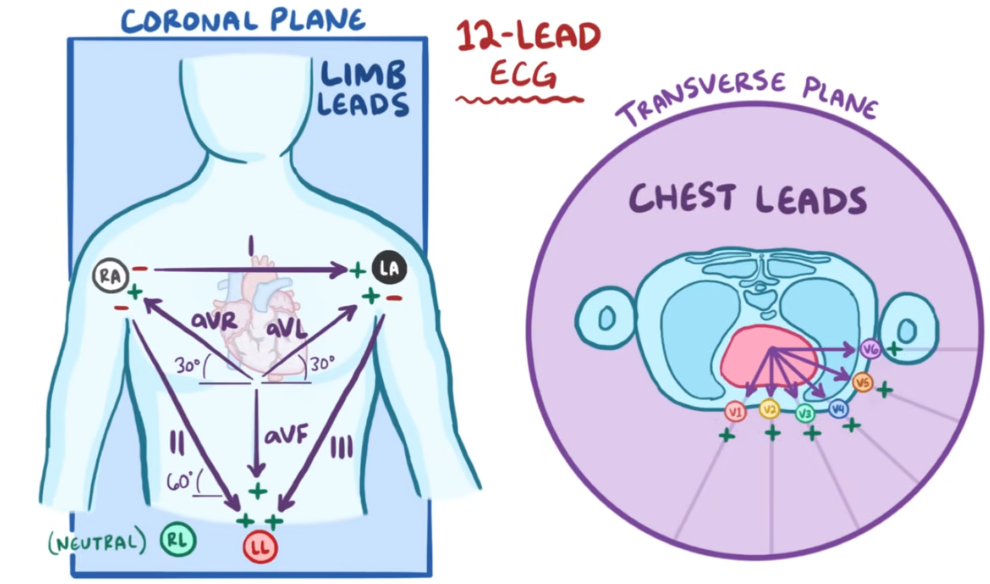
\includegraphics[width=0.7\linewidth]{images/pos-elettrodi.png}
    \caption{Posiziamento degli elettrodi}
    \label{fig:placeholder}
\end{figure}

\begin{itemize}
    \item \textbf{V1-V6}: sono i grafi generati dai sei elettrodi precordiali, numerati dal mediastino (V1) alla parte laterale del corpo (V6).  
    \item \textbf{aVR}: grafo proveniente dal braccio destro (polso o spalla).
    \item \textbf{aVL}: grafo proveniente dal braccio sinistro. (polso o spalla).
    \item \textbf{aVF}: grafo proveniente dal piede sinistro (caviglia o gamba).
    \item \textbf{I}: utilizza il braccio destro come polo negativo e il braccio sinistro come polo positivo.
    \item \textbf{II}: utilizza il braccio destro come polo negativo e il piede sinistro come polo positivo.
    \item \textbf{III}: utilizza il braccio sinistro come polo negativo e il piede sinistro come polo positivo.
\end{itemize}
L'elettrodo nel piede destro viene utilizzato dall'elettrocardiografo per minimizzare il rumore e ridurre le interferenze elettriche, come fosse la massa di un circuito elettrico.

\subsection{Calcolo delle Derivazioni}
Le dodici derivazioni dell'ECG non sono tutte ottenute allo stesso modo: si distinguono infatti le \textit{derivazioni bipolari}, teorizzate da Einthoven, le \textit{derivazioni unipolari aumentate}, teorizzate da Goldberger.

\subsubsection{Derivazioni pericordiali}
Le derivazioni \textit{V1-V6} utilizzano un punto di riferimento comune, a potenziale zero, chiamato \textit{terminale centrale di Wilson}: viene calcolato come la media dei tre elettrodi periferici, escludendo il piede destro.

\subsubsection{Derivazioni di Einthoven}
Le derivazioni \textit{I}, \textit{II} e \textit{III} costituiscono il cosiddetto \textbf{triangolo di Einthoven}: i tre elettrodi periferici (braccio destro, braccio sinistro e piede sinistro) vengono idealmente collegati tra loro a formare un triangolo equilatero, con il cuore posizionato al centro. Ogni derivazione misura la differenza di potenziale tra una coppia di elettrodi (da cui il termine \textit{bipolare}):
\begin{itemize}
    \item \textbf{I} = braccio sinistro (+) $-$ braccio destro ($-$)
    \item \textbf{II} = piede sinistro (+) $-$ braccio destro ($-$)
    \item \textbf{III} = piede sinistro (+) $-$ braccio sinistro ($-$)
\end{itemize}
Dalla geometria del triangolo discende la cosiddetta \textbf{legge di Einthoven}, secondo cui la somma algebrica delle derivazioni I e III è pari alla derivazione II:
\[
I + III = II
\]
Questa relazione è utile anche come controllo di coerenza del tracciato registrato.

\subsubsection{Derivazioni di Goldberger}
Le derivazioni \textit{aVR}, \textit{aVL} e \textit{aVF} sono invece \textit{unipolari}: misurano il potenziale di un singolo elettrodo periferico rispetto a un riferimento comune, chiamato \textit{terminale centrale}. Goldberger propose di costruire tale riferimento come media dei due elettrodi periferici diversi da quello esplorato, escludendo però quest'ultimo dal calcolo del riferimento stesso. Questo accorgimento fa sì che il segnale ottenuto risulti amplificato del 50\% rispetto a quanto si otterrebbe usando il \textit{terminale centrale di Wilson} (media di tutti e tre gli elettrodi periferici), da cui il prefisso "a" nel nome:
\begin{itemize}
    \item \textbf{aVR} (\textit{augmented Vector Right}): esplora il braccio destro.
    \item \textbf{aVL} (\textit{augmented Vector Left}): esplora il braccio sinistro.
    \item \textbf{aVF} (\textit{augmented Vector Foot}): esplora il piede sinistro.
\end{itemize}

Le sei derivazioni periferiche (I, II, III, aVR, aVL, aVF), pur derivando dagli stessi tre elettrodi fisici, osservano il cuore secondo angolazioni diverse sul piano frontale, distanziate tra loro di 30°: è proprio questa disposizione angolare a essere riorganizzata nel sistema Cabrera descritto più avanti.
\begin{figure}[h!]
    \centering
    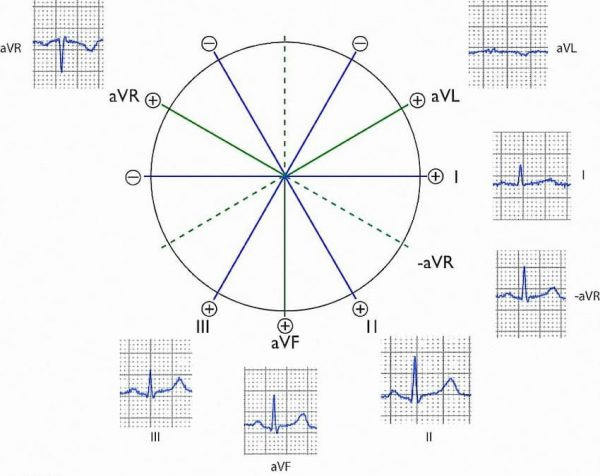
\includegraphics[width=0.7\linewidth]{images/visione_core.jpg}
    \caption{Viste prospettiche del cuore rispetto a Einthoven e Goldberger}
    \label{fig:vista_cuore}
\end{figure}

\subsection{Visibilità}

L'ECG a 12 derivazioni consente una buona visione del cuore offrendo una copertura complessiva di tutte le pareti cardiache. Le derivazioni inferiori (II, III, aVF) esplorano la parete inferiore, le derivazioni laterali (I, aVL, V5, V6) la parete laterale, mentre le derivazioni precordiali (V1--V4) forniscono informazioni sulla parete anteriore e sul setto interventricolare.

Ne consegue che alcune regioni risultano scarsamente rappresentate nella configurazione standard, come la parete posteriore e il ventricolo destro, che richiedono derivazioni aggiuntive per una valutazione completa.

Per questa ragione, le derivazioni di questa tipologia di ECG vengono tradizionalmente organizzate e interpretate in funzione della visione del ventricolo sinistro: ciascun gruppo di derivazioni corrisponde a una parete specifica di tale ventricolo, consentendo una lettura ordinata per regioni anatomiche. È proprio su questo principio che si fonda il sistema Cabrera, che propone una riorganizzazione delle derivazioni frontali secondo una sequenza anatomicamente continua relativamente all'angolo di osservazione del ventricolo, con l'obiettivo di rendere più intuitiva l'interpretazione dell'attività elettrica del ventricolo sinistro.

\begin{figure}[h!]
    \centering
    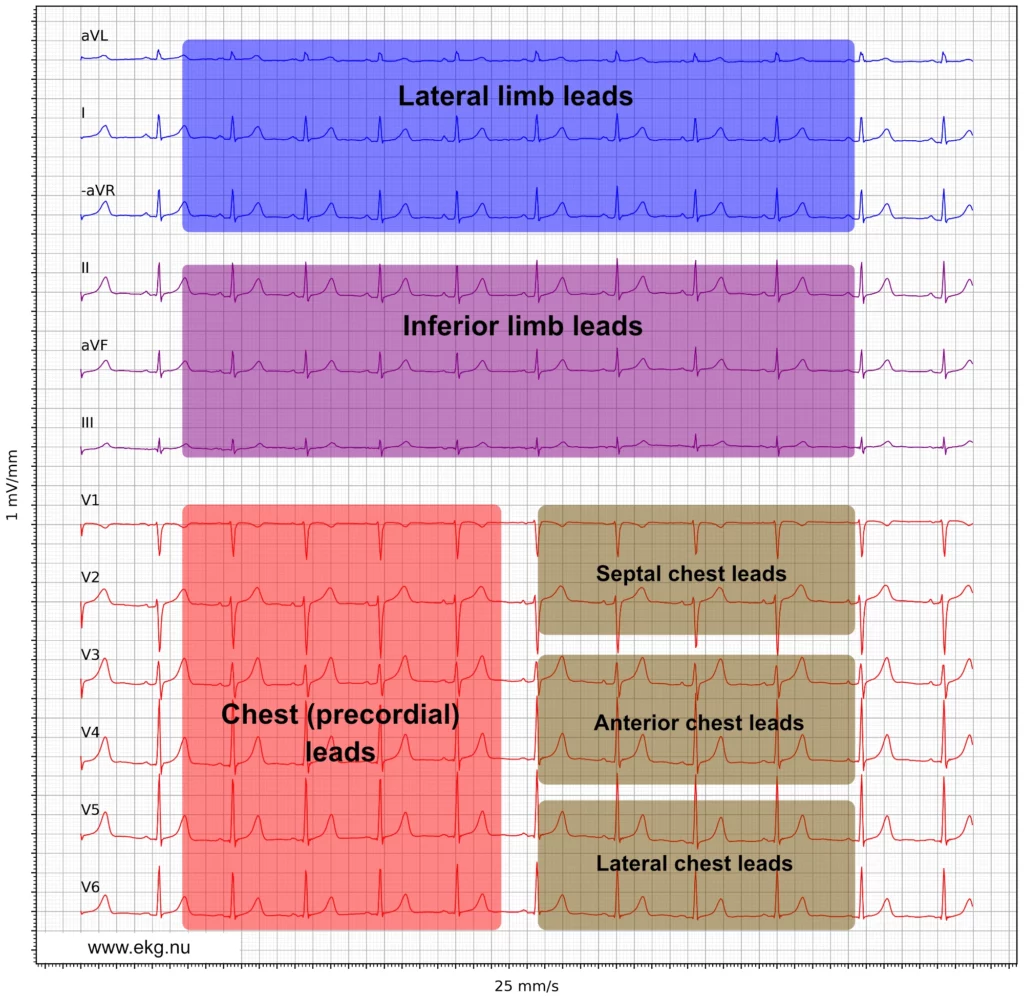
\includegraphics[width=0.50\linewidth]{images/12-lead-ecg-leads-limb-chest-cabrera.png}
    \caption{Sistema Cabrera}
    \label{fig:placeholder}
\end{figure}

\subsection{Lettura ECG}
L'elettrocardiografo presenta un diagramma per ogni derivazione. La differenza di potenziale, espressa in $mV$, è rappresentata sull'asse Y, mentre il tempo è rappresentato sull'asse delle X. L'ECG viene stampato su carta millimetrata caratterizzata da piccoli quadrati da un $mm$ di lato (riga fine) e grandi quadrati d $5\,mm$ di lato (riga spessa); in un elettrocardiografo ben calibrato e con velocità di stampa standard a $25\,mm/s$, avremo che $10\,mm$ (due blocchi grandi) sull'asse Y corrispondono ad $1\,mV$, e $10\,mm$ sull'asse delle X equivalgono a $400\,ms$.
 Le fasi della contrazione cardiaca si presentano nell'ECG tramite un pattern ricorrente di diverse onde: la prima, chiamata \textbf{onda P}, rappresenta la depolarizzazione atriale, l’evento elettrico che innesca e precede la contrazione meccanica (sistole) atriale, ed è solitamente visibile nella maggior parte delle derivazioni; poi abbiamo il \textbf{complesso QRS}, che rappresenta la depolarizzazione ventricolare, l’evento elettrico che precede e innesca la sistole ventricolare, ed è composto da tre deflessioni distinte: l'\textit{onda Q} (prima deflessione negativa) data dalla depolarizzazione del setto interventricolare, l'\textit{onda R} (deflessione positiva principale) data dalla depolarizzazione delle pareti "libere", essendo il ventricolo sinistro con massa muscolare maggiore, il suo vettore predomina, infine abbiamo l'\textit{onda S} (seconda deflessione negativa) data dalla depolarizzazione alla base dei ventricoli, cioè nella parte alta, vicino ai grandi vasi. Il complesso QRS è di maggiore ampiezza e durata rispetto all'onda P, a indicare la maggiore massa muscolare dei ventricoli. Segue il \textbf{segmento ST}, un breve tratto isoelettrico che avviene tra la fine della depolarizzazione ventricolare e l'inizio della ripolarizzazione; in condizioni fisiologiche si trova sulla linea di base. Infine, l'\textbf{onda T} rappresenta la ripolarizzazione ventricolare, ovvero il ritorno delle cellule miocardiche allo stato di riposo in preparazione al ciclo successivo; è normalmente positiva nelle derivazioni in cui il complesso QRS presenta una deflessione principale positiva.

Ovviamente, la visibilità e la direzione delle onde non saranno le stesse per tutte le derivazioni perché, come detto in precedenza, gli elettrodi misurano i campi elettrici direzionati verso di essi. Quindi ogni derivazione mostrerà diversi aspetti del ciclo cardiaco, ad esempio, in V1 l'onda R è minuscola e la S è profonda mentre in V5-V6 è l'opposto, l'onda R è alta e la S è quasi assente.

\begin{figure}[h!]
    \centering
    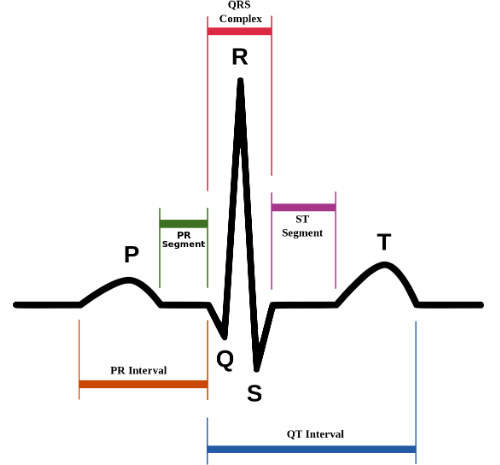
\includegraphics[width=0.4\linewidth]{images/onda-pqrst.jpg}
    \caption{onda P QRS T}
    \label{fig:placeholder}
\end{figure}

Tra le onde è possibile misurare alcuni \textbf{intervalli} di rilevanza clinica. L'\textbf{intervallo PR}, misurato dall'inizio dell'onda P all'inizio del complesso QRS, riflette il tempo di conduzione atrioventricolare, ovvero il ritardo fisiologico introdotto dal nodo atrioventricolare prima che l'impulso raggiunga i ventricoli; il suo valore normale è compreso tra $120$ e $200\,ms$. L'\textbf{intervallo QT}, misurato dall'inizio del complesso QRS alla fine dell'onda T, rappresenta la durata complessiva della sistole elettrica ventricolare, comprensiva sia della depolarizzazione che della ripolarizzazione; poiché dipende dalla frequenza cardiaca, viene spesso corretto con apposite formule (QTc) e il suo valore normale è generalmente inferiore a $440\,ms$ nell'uomo e $460\,ms$ nella donna.

\subsubsection{Ritmo sinusale normale}
Viene definito \textbf{ritmo sinusale normale} un ritmo cardiaco in cui ogni impulso ha origine regolarmente dal nodo senoatriale, si propaga attraverso il sistema di conduzione in modo fisiologico e produce sull'ECG un pattern caratteristico e ripetitivo. È importante precisare che la presenza di un ritmo sinusale normale indica esclusivamente la corretta origine e conduzione dell'impulso elettrico, non escludendo la presenza di patologie strutturali o funzionali del cuore.

I criteri che definiscono questo ritmo sono i seguenti:
\begin{itemize}
    \item Ogni complesso QRS deve essere preceduto da un'onda P
    \item L'intervallo PR deve essere costante e compreso tra $120$ e $200\,ms$
    \item La frequenza cardiaca deve essere compresa tra $60$ e $100$ battiti al minuto
    \item I complessi QRS devono essere regolarmente distanziati tra loro
    \item L'onda P deve essere positiva in $I$ e $II$, e negativa in $aVR$  
\end{itemize}
